% COMPILATION REQUIREMENTS:
% 1. Compile with XeLaTeX (or LuaLaTeX) to support the custom 'Inter' font.
%    Command: xelatex presentation.tex
% 2. Required packages (standard in TeX Live / MiKTeX):
%    - beamer, tikz, tcolorbox, fontspec, xcolor, graphicx
%
% 3. IMAGE PLACEHOLDERS: 
%    To finalize this deck, replace the \demoPlaceholder{...} commands 
%    with \includegraphics[width=\textwidth]{real_screenshot.png} 
%    pointing to your actual application screenshots.

\documentclass[aspectratio=169, xcolor=table]{beamer}

% Packages
\usepackage{fontspec}
\usepackage{tikz}
\usepackage[most]{tcolorbox}
\usepackage{graphicx}
\usepackage{calc}

% -------------------------------------------------------------------------
% TYPOGRAPHY
% -------------------------------------------------------------------------
% SentinelAI uses 'Inter' as its primary font.
% If Inter is not installed on your system, XeLaTeX will fall back or throw an error.
% You can download it from fonts.google.com or comment this out to use the default sans.
\IfFontExistsTF{Inter}{
    \setmainfont{Inter}
    \setsansfont{Inter}
}{
    % Fallback if Inter is missing
    \renewcommand{\familydefault}{\sfdefault}
}

% -------------------------------------------------------------------------
% EXTRACTED DESIGN TOKENS (from user_frontend globals.css & frontend globals.css)
% -------------------------------------------------------------------------
\definecolor{SentinelBg}{HTML}{0A0A0A}         % --color-bg: #0a0a0a
\definecolor{SentinelSurface}{HTML}{141414}    % --color-surface: #141414
\definecolor{SentinelSurfaceRaised}{HTML}{1C1C1C} % --color-surface-raised: #1c1c1c
\definecolor{SentinelAccent}{HTML}{CDFF50}     % --color-accent: #cdff50
\definecolor{SentinelText}{HTML}{FFFFFF}       % --color-text-primary: #ffffff
\definecolor{SentinelTextSec}{HTML}{A0A0A0}    % --color-text-secondary: #a0a0a0
\definecolor{SentinelDanger}{HTML}{E53E3E}     % --color-danger: #e53e3e
\definecolor{SentinelSuccess}{HTML}{48BB78}    % --color-success: #48bb78

% -------------------------------------------------------------------------
% CUSTOM BEAMER THEME
% -------------------------------------------------------------------------
\setbeamercolor{background canvas}{bg=SentinelBg}
\setbeamercolor{normal text}{fg=SentinelText}
\setbeamercolor{title}{fg=SentinelText}
\setbeamercolor{frametitle}{fg=SentinelText}
\setbeamercolor{item}{fg=SentinelAccent}
\setbeamercolor{itemize item}{fg=SentinelAccent}
\setbeamercolor{itemize subitem}{fg=SentinelAccent}
\setbeamercolor{itemize subsubitem}{fg=SentinelAccent}

% Remove navigation symbols
\setbeamertemplate{navigation symbols}{}

% Custom Frame Title
\setbeamertemplate{frametitle}{
    \vspace{0.4cm}
    \begin{beamercolorbox}[wd=\paperwidth,leftskip=0.8cm]{frametitle}
        \usebeamerfont{frametitle}\textbf{\insertframetitle}
    \end{beamercolorbox}
}

% Custom Footer
\setbeamertemplate{footline}{
    \leavevmode%
    \hbox{%
    \begin{beamercolorbox}[wd=\paperwidth,ht=2.25ex,dp=1ex,leftskip=0.8cm,rightskip=0.8cm]{}%
        \textcolor{SentinelTextSec}{\small SentinelAI} \hfill \textcolor{SentinelTextSec}{\small \insertframenumber}
    \end{beamercolorbox}}%
    \vskip4pt%
}

% -------------------------------------------------------------------------
% CUSTOM UI ELEMENTS (TCOLORBOX for glassmorphism/card UI)
% -------------------------------------------------------------------------
\tcbset{
    sentinelcard/.style={
        colback=SentinelSurface,
        colframe=SentinelSurfaceRaised,
        boxrule=1pt,
        arc=4mm,       % matches rounded-14px / rounded-xl
        auto outer arc,
        coltext=SentinelText,
        left=4mm, right=4mm, top=4mm, bottom=4mm,
        fonttitle=\bfseries,
        coltitle=SentinelText
    },
    sentinelpill/.style={
        colback=SentinelAccent,
        colframe=SentinelAccent,
        coltext=SentinelBg,
        arc=2mm,
        boxrule=0pt,
        top=1mm, bottom=1mm, left=3mm, right=3mm,
        fontupper=\bfseries\small,
        halign=center
    }
}

% Macro for a placeholder image
\newcommand{\demoPlaceholder}[2]{
    \begin{tcolorbox}[colback=SentinelSurfaceRaised, colframe=SentinelSurfaceRaised, arc=4mm, height=#1, valign=center, halign=center]
        \textcolor{SentinelTextSec}{\Large \textit{[Placeholder: #2]}} \\
        \vspace{2mm}
        \textcolor{SentinelTextSec}{\small (Replace with actual screenshot)}
    \end{tcolorbox}
}

% -------------------------------------------------------------------------
% DOCUMENT START
% -------------------------------------------------------------------------
\begin{document}

% -------------------------------------------------------------------------
% SLIDE 1: TITLE
% -------------------------------------------------------------------------
\begin{frame}[plain]
    \begin{center}
        \vspace*{1.5cm}
        {\Huge \textbf{\textcolor{SentinelAccent}{Sentinel}AI}} \\
        \vspace{0.4cm}
        {\Large AI-Powered Incident Intelligence \& Resource Command Platform} \\
        \vspace{1.5cm}
        
        \begin{tcolorbox}[sentinelcard, width=0.8\textwidth, center, colback=SentinelBg, colframe=SentinelSurfaceRaised]
            \centering
            \textcolor{SentinelTextSec}{\textbf{TEAM [TEAM NAME HERE]}} \\
            \vspace{0.3cm}
            % EMPTY NAME SLOTS FOR REAL NAMES
            [Name 1] \quad $\bullet$ \quad [Name 2] \quad $\bullet$ \quad [Name 3] \quad $\bullet$ \quad [Name 4]
        \end{tcolorbox}
    \end{center}
\end{frame}

% -------------------------------------------------------------------------
% SLIDE 2: THE PROBLEM
% -------------------------------------------------------------------------
\begin{frame}{The Problem: Reactive \& Blind Operations}
    \vspace{0.5cm}
    \begin{columns}[T]
        \begin{column}{0.48\textwidth}
            \begin{tcolorbox}[sentinelcard, height=5.5cm]
                \textcolor{SentinelDanger}{\textbf{1. Blind Resource Allocation}}
                \vspace{0.2cm}
                \begin{itemize}
                    \item Dispatching to the \textit{nearest} station, not the most \textit{ready} station.
                    \item Leads to overloaded units while others sit idle.
                \end{itemize}
                \vspace{0.4cm}
                
                \textcolor{SentinelDanger}{\textbf{2. Lost City Memory}}
                \vspace{0.2cm}
                \begin{itemize}
                    \item Millions of past logs, but zero real-time learning.
                    \item Every incident is handled from scratch.
                \end{itemize}
            \end{tcolorbox}
        \end{column}
        
        \begin{column}{0.48\textwidth}
            \begin{tcolorbox}[sentinelcard, height=5.5cm]
                \textcolor{SentinelDanger}{\textbf{3. Late Hotspot Detection}}
                \vspace{0.2cm}
                \begin{itemize}
                    \item Traffic corridors decay into gridlock before operators notice the pattern.
                \end{itemize}
                \vspace{0.4cm}
                
                \textcolor{SentinelDanger}{\textbf{4. Event-Driven Chaos}}
                \vspace{0.2cm}
                \begin{itemize}
                    \item Planned events (VIPs, rallies) cause unexpected congestion because impact isn't simulated in advance.
                \end{itemize}
            \end{tcolorbox}
        \end{column}
    \end{columns}
\end{frame}

% -------------------------------------------------------------------------
% SLIDE 3: THE VISION
% -------------------------------------------------------------------------
\begin{frame}{The Vision}
    \begin{center}
        {\Large \textbf{An AI Copilot for traffic control rooms, from report to resolution.}}
    \end{center}
    \vspace{0.8cm}
    
    \begin{center}
    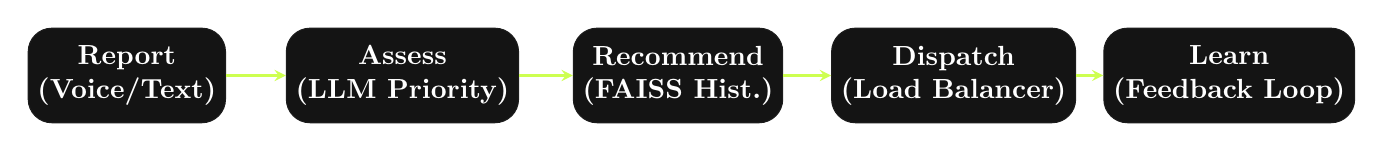
\begin{tikzpicture}[
        box/.style={draw=SentinelSurfaceRaised, fill=SentinelSurface, text=SentinelText, 
                    rounded corners=3mm, minimum height=1.2cm, minimum width=2.4cm, align=center, font=\bfseries},
        arrow/.style={->, thick, SentinelAccent, >=stealth}
    ]
        \node[box] (n1) at (0,0) {Report\\(Voice/Text)};
        \node[box] (n2) at (3.5,0) {Assess\\(LLM Priority)};
        \node[box] (n3) at (7,0) {Recommend\\(FAISS Hist.)};
        \node[box] (n4) at (10.5,0) {Dispatch\\(Load Balancer)};
        \node[box] (n5) at (14,0) {Learn\\(Feedback Loop)};
        
        \draw[arrow] (n1) -- (n2);
        \draw[arrow] (n2) -- (n3);
        \draw[arrow] (n3) -- (n4);
        \draw[arrow] (n4) -- (n5);
    \end{tikzpicture}
    \end{center}
\end{frame}

% -------------------------------------------------------------------------
% SLIDE 4: SYSTEM ARCHITECTURE
% -------------------------------------------------------------------------
\begin{frame}{System Architecture}
    \vspace{0.2cm}
    \begin{center}
    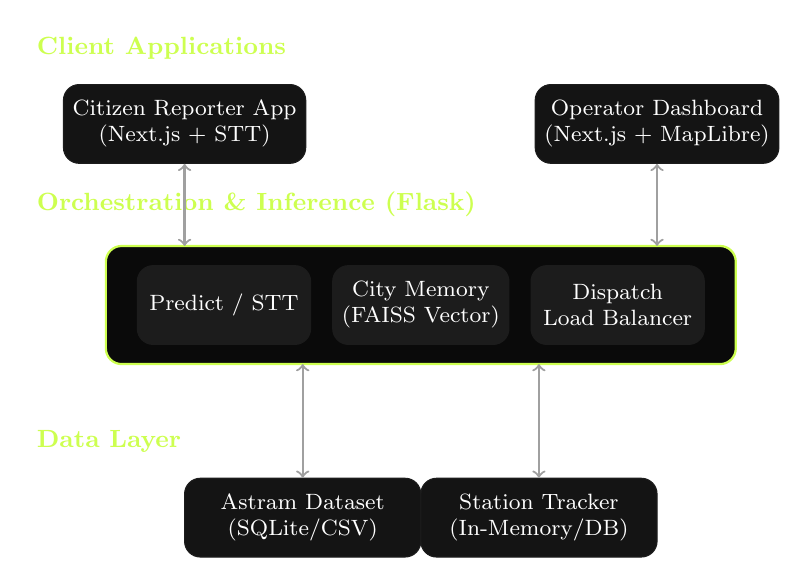
\begin{tikzpicture}[
        layer/.style={draw=SentinelSurfaceRaised, fill=SentinelSurface, rounded corners=2mm, minimum height=1cm, text=SentinelText, align=center, font=\footnotesize},
        lbl/.style={font=\bfseries\small, text=SentinelAccent, anchor=south west}
    ]
        % Frontend Layer
        \node[lbl] at (-5, 2.5) {Client Applications};
        \node[layer, minimum width=3cm] (citizen) at (-3, 1.8) {Citizen Reporter App\\(Next.js + STT)};
        \node[layer, minimum width=3cm] (dashboard) at (3, 1.8) {Operator Dashboard\\(Next.js + MapLibre)};
        
        % Core API Layer
        \node[lbl] at (-5, 0.5) {Orchestration \& Inference (Flask)};
        \node[layer, minimum width=8cm, minimum height=1.5cm, fill=SentinelBg, draw=SentinelAccent, thick] (api) at (0, -0.5) {};
        
        \node[layer, fill=SentinelSurfaceRaised, minimum width=2.2cm] (predict) at (-2.5, -0.5) {Predict / STT};
        \node[layer, fill=SentinelSurfaceRaised, minimum width=2.2cm] (faiss) at (0, -0.5) {City Memory\\(FAISS Vector)};
        \node[layer, fill=SentinelSurfaceRaised, minimum width=2.2cm] (dispatch) at (2.5, -0.5) {Dispatch\\Load Balancer};
        
        % Storage Layer
        \node[lbl] at (-5, -2.5) {Data Layer};
        \node[layer, minimum width=3cm] (db) at (-1.5, -3.2) {Astram Dataset\\(SQLite/CSV)};
        \node[layer, minimum width=3cm] (redis) at (1.5, -3.2) {Station Tracker\\(In-Memory/DB)};
        
        % Connections
        \draw[<->, thick, SentinelTextSec] (citizen) -- (-3, 0.25);
        \draw[<->, thick, SentinelTextSec] (dashboard) -- (3, 0.25);
        \draw[<->, thick, SentinelTextSec] (-1.5, -1.25) -- (db);
        \draw[<->, thick, SentinelTextSec] (1.5, -1.25) -- (redis);
    \end{tikzpicture}
    \end{center}
\end{frame}

% -------------------------------------------------------------------------
% SLIDE 5: AI COPILOT & CITY MEMORY ENGINE
% -------------------------------------------------------------------------
\begin{frame}{AI Incident Copilot + City Memory Engine}
    \begin{columns}[T]
        \begin{column}{0.4\textwidth}
            \begin{tcolorbox}[sentinelcard]
                \textbf{Real-Time Assessment}
                \begin{itemize}
                    \item LLM extracts priority, vehicle types, and estimates resolution time instantly.
                    \item Eliminates manual tagging.
                \end{itemize}
            \end{tcolorbox}
            \begin{tcolorbox}[sentinelcard]
                \textbf{City Memory Engine}
                \begin{itemize}
                    \item Queries FAISS vector DB for similar historical events.
                    \item Displays the most common outcomes and average clearance times from the past.
                \end{itemize}
            \end{tcolorbox}
        \end{column}
        
        \begin{column}{0.55\textwidth}
            % Replace with screenshot of the left column of IncidentDetailPage
            \demoPlaceholder{6.5cm}{Incident Detail / Historical Similar Cases}
        \end{column}
    \end{columns}
\end{frame}

% -------------------------------------------------------------------------
% SLIDE 6: STATION LOAD BALANCER
% -------------------------------------------------------------------------
\begin{frame}{Station Load Balancer \& Dispatch}
    \begin{columns}[T]
        \begin{column}{0.4\textwidth}
            \begin{tcolorbox}[sentinelcard]
                \textbf{Not just "nearest". Most Ready.}
                \vspace{0.3cm}
                
                \small
                The \textbf{Readiness Score (0-100)} dynamically weights:
                \begin{itemize}
                    \item Available Officers \& Vehicles
                    \item Current Active Incidents
                    \item Historical Efficiency
                \end{itemize}
                \vspace{0.3cm}
                
                \textbf{Dynamic Resource Engine} calculates exact manpower/barricade needs based on the incident heuristics (e.g. heavy vehicles).
            \end{tcolorbox}
        \end{column}
        
        \begin{column}{0.55\textwidth}
            % Replace with screenshot of the Green "Recommended Station" Panel
            \demoPlaceholder{6.5cm}{Recommended Station \& Readiness Panel}
        \end{column}
    \end{columns}
\end{frame}

% -------------------------------------------------------------------------
% SLIDE 7: CORRIDOR RIPPLE SIMULATOR
% -------------------------------------------------------------------------
\begin{frame}{The "Wow" Factor: Corridor Ripple Simulator}
    \begin{columns}[T]
        \begin{column}{0.45\textwidth}
            \vspace{0.5cm}
            {\Large \textbf{Traffic behaves like fluid dynamics.}}
            \vspace{0.4cm}
            
            \begin{tcolorbox}[sentinelcard]
                \begin{itemize}
                    \item We don't just view the incident; we predict the \textbf{blast radius}.
                    \item \textbf{Breadth-First Search (BFS)} algorithm calculates ripple propagation.
                    \item Visualizes downstream intersection impacts dynamically on the map.
                    \item Enables preemptive barricade deployment \textit{before} gridlock hits.
                \end{itemize}
            \end{tcolorbox}
        \end{column}
        
        \begin{column}{0.5\textwidth}
            % Replace with screenshot of the BengaluruMap showing red pulsing ripple nodes
            \demoPlaceholder{6.5cm}{Ripple Simulator on 3D Map}
        \end{column}
    \end{columns}
\end{frame}

% -------------------------------------------------------------------------
% SLIDE 8: EVENT-DRIVEN CONGESTION COVERAGE
% -------------------------------------------------------------------------
\begin{frame}{Proactive Event-Driven Congestion}
    \begin{columns}[T]
        \begin{column}{0.4\textwidth}
            \begin{tcolorbox}[sentinelcard]
                \textbf{Not Just Reactive}
                \begin{itemize}
                    \item Most systems only react to accidents. SentinelAI anticipates planned events.
                    \item Logs VIP movements, processions, and protests.
                    \item Generates an \textbf{Impact Forecast} based on expected scale and historical precedents.
                \end{itemize}
            \end{tcolorbox}
        \end{column}
        
        \begin{column}{0.55\textwidth}
            % Replace with screenshot of the "Log Planned Event" forecast UI
            \demoPlaceholder{6.5cm}{Planned Event Impact Forecast UI}
        \end{column}
    \end{columns}
\end{frame}

% -------------------------------------------------------------------------
% SLIDE 9: WHY THIS WINS
% -------------------------------------------------------------------------
\begin{frame}{Why SentinelAI Wins}
    \vspace{0.5cm}
    \begin{columns}[T]
        \begin{column}{0.31\textwidth}
            \begin{tcolorbox}[sentinelcard, height=4.5cm, halign=center]
                \textcolor{SentinelAccent}{\Large \textbf{Data-Driven Dispatch}}
                \vspace{0.3cm}
                
                \small
                Moves away from rudimentary proximity models to a holistic \textbf{Readiness Score}, eliminating station burnout.
            \end{tcolorbox}
        \end{column}
        \begin{column}{0.31\textwidth}
            \begin{tcolorbox}[sentinelcard, height=4.5cm, halign=center]
                \textcolor{SentinelAccent}{\Large \textbf{Anticipatory AI}}
                \vspace{0.3cm}
                
                \small
                Simulates ripple effects and forecasts planned event impacts \textit{before} congestion paralyzes the corridor.
            \end{tcolorbox}
        \end{column}
        \begin{column}{0.31\textwidth}
            \begin{tcolorbox}[sentinelcard, height=4.5cm, halign=center]
                \textcolor{SentinelAccent}{\Large \textbf{Zero Friction}}
                \vspace{0.3cm}
                
                \small
                Multilingual STT voice reporting for citizens, combined with one-click automated resource allocation for operators.
            \end{tcolorbox}
        \end{column}
    \end{columns}
\end{frame}

% -------------------------------------------------------------------------
% SLIDE 10: CLOSING
% -------------------------------------------------------------------------
\begin{frame}[plain]
    \begin{center}
        \vspace*{2cm}
        {\Huge \textbf{Thank You.}} \\
        \vspace{0.5cm}
        {\Large SentinelAI is ready for deployment.} \\
        \vspace{1.5cm}
        
        \begin{tcolorbox}[sentinelcard, width=0.6\textwidth, center]
            \centering
            \textbf{Next Steps on the Roadmap:} \\
            \vspace{0.2cm}
            \small
            1. Expanding to city-wide dynamic graph edges \\
            2. V2 CCTV feed ingestion \\
            3. Automated SMS alerts for local residents
        \end{tcolorbox}
    \end{center}
\end{frame}

\end{document}
